\section{Introduction}
    The objective of this exercise is to study simple harmonic oscillation, including how to find the spring constant, how to analyze the relationship between the oscillation period and the mass of the oscillator, whether the oscillation period depends on the amplitude. Besides, the relationship between the maximum speed and the amplitude will also be examined.\\
    Simple harmonic motion is one of the most fundamental periodic motions, where the restoring force is proportional to the displacement from the equilibrium position so that the position of a particle depends on time as a sine (or cosine) function.\\
\subsection{Hooke's law}
    Within the elastic limit of deformation, the force $F_x$ needed to compress or strech a spring is proportional to the distance, \emph{i.e.},
    \begin{equation}
        \label{hooke}
        F_x=kx,
    \end{equation}
    where $k$, the spring constant, characterizing how easy to deform a spring. We use \emph{Jolly balance} in this exercise to find that constant. The relation \ref{hooke} is known as the \emph{Hooke's Law}. Therefore, the elastic force is found according to Newton's third law of dynamics, whose magnitude is the same but direction is opposite. It's also known as restoring forceas it always tries to restore the system back to the equilibrium.\\

\subsection{Equation of Motion of the Simple Harmonic Oscillator}
    \begin{figure}[htbp]
        \label{massspring}
        \centering
        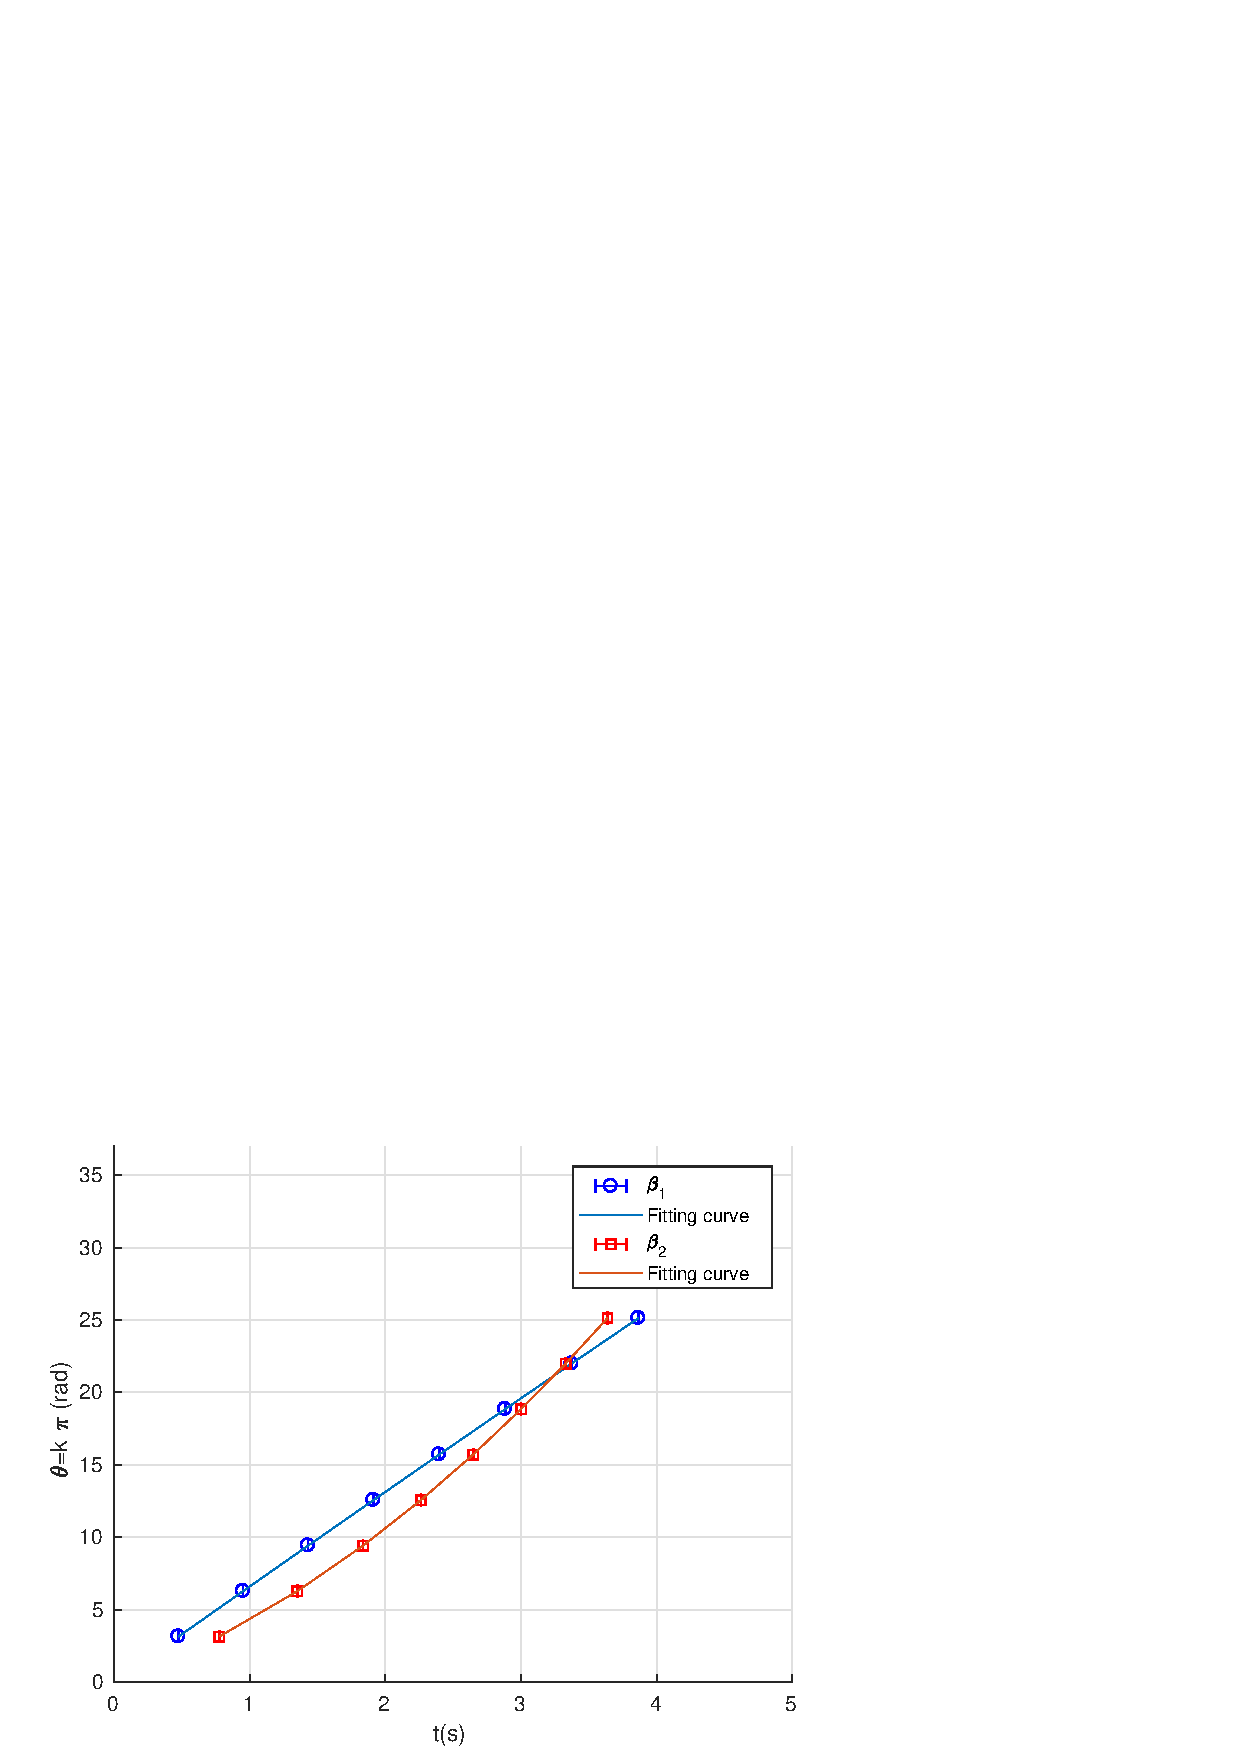
\includegraphics[height=0.6in]{images/1.png}
        \caption{Mass-spring system}
    \end{figure}

    As shown in Figure \ref{massspring}, the mass with two springs is placed on an air track, which aims at eliminating the frictional forces. Assuming that the restoring force is the only force acting on mass M, the equation of motion od mass M is
    \begin{equation}
        \label{diff}
        M\frac{d^2x}{dt^2}+(k_1+k_2)x=0.
    \end{equation}
    Hence the general solution to Eq. \ref{diff} is
    \begin{equation}
        x(t)=Acos(\omega_0t+\phi_0),
    \end{equation}
    where $\omega_0=\sqrt{(k_1+k_2)/M}$ is the natural angular frequency of the oscillations (determined by the parameters of the system), A is the amplitude, and $\phi_0$ is the initial phase (determined by initial conditions). The natural period of oscillation is
    \begin{equation}
        T=\frac{2\pi}{\omega_0}=2\pi\sqrt{\frac{M}{k_1+k_2}}.
    \end{equation}\\
    
    In this exercise, the relationship mentioned above will be studied.\\
    
\subsection{Mass of the Spring}
    We take into the mass of the springs in terms of the so-called \emph{effective mass}, which is the sum of the mass of the object $M$ and the effective mass of springs $m_0$. The angular frequency can be expressed as
    \begin{equation}
        \omega_0=\sqrt{\frac{k_1+k_2}{M+m_0}}
    \end{equation}
    where $m_0$ is 1/3 of the actual mass of the spring.

\subsection{Mechanical Energy in Harmonic Motion}
    The elastic potential energy for a spring-mass system is $U=kx^2/2$ and the kinetic energy of an oscillating mass is $K=mv^2/2$.    
    At the equilibrium position ($x=0$), the speed of the mass is maximum $v=v_{max}$. At this point the total mechanical energy is equal to maximum kinetic energy $K_{max}$ . On the other hand, at maximum displacement ($x=\pm A$) the mass is instantaneously at rest, and the contribution to the total mechanical energy is due to the potential energy only, which is at its maximum $U_{max}$. In the absence of non-conservative forces (such as frictional forces or drag forces), the total mechanical energy is conserved and $K_{max}=U_{max}$, which implies
    \begin{equation}
        k=\frac{mv_{max}^2}{A^2}.
    \end{equation}

